\documentclass[12pt]{article}
\usepackage{latexblog}

% ============================================================
% Blog Metadata
% ============================================================
\blogtitle{PyQt5入门小程序}
\blogdate{2020-05-13}
\blogtags{框架, Python, Qt, 闲话编程}
\bloglang{zh}
\blogsummary{}

\begin{document}
\makeblogtitle

最近有非计算机专业的同学想学PyQT，但是又不知道怎么搞，所以我做了一个简单的例子。这个例子是一个简单的图片显示器。这是一篇写给新人的入门文章，希望有所帮助。

\section{Qt程序的基本结构}\label{qtux7a0bux5e8fux7684ux57faux672cux7ed3ux6784}

跟其他程序一样，所有的程序都会有一个主入口，然后一行一行的调用代码，而GUI程序跟其他程序有一个区别就是，只有你显示的关闭界面，程序才会退出。所以整个GUI的程序大致会是这样一个原理（下面是伪代码，不是实际的程序）：

\begin{Shaded}
\begin{Highlighting}[]
\DataTypeTok{void} \FunctionTok{main}\OperatorTok{()} \OperatorTok{\{}
    \ControlFlowTok{while}\OperatorTok{(}\KeywordTok{true}\OperatorTok{)} \OperatorTok{\{}
\NormalTok{        command }\OperatorTok{=} \FunctionTok{fetch\_user\_input\_event}\OperatorTok{()}
        \ControlFlowTok{if}\OperatorTok{(}\NormalTok{command }\OperatorTok{==}\NormalTok{ quit}\OperatorTok{):}
            \FunctionTok{exit}\OperatorTok{();}
        \ControlFlowTok{else}
\NormalTok{            keep\_rendering\_ui}
    \OperatorTok{\}}
\OperatorTok{\}}
\end{Highlighting}
\end{Shaded}

然而实际上不需要我们去操心这个，Qt框架会帮我们处理这个逻辑，一个Qt应用就是这样：

\begin{Shaded}
\begin{Highlighting}[]
\KeywordTok{def}\NormalTok{ main():}
\NormalTok{    app }\OperatorTok{=}\NormalTok{ QApplication(sys.argv)}
\NormalTok{    window }\OperatorTok{=}\NormalTok{ MainWindow()}
\NormalTok{    window.show()         }\CommentTok{\# 必须显示的调用，显示一个界面}
\NormalTok{    app.exec\_()           }\CommentTok{\# 等待程序退出，否则界面一闪而过}

\ControlFlowTok{if} \VariableTok{\_\_name\_\_} \OperatorTok{==} \StringTok{\textquotesingle{}\_\_main\_\_\textquotesingle{}}\NormalTok{:}
\NormalTok{    main()}
\end{Highlighting}
\end{Shaded}

\section{UI绘制}\label{uiux7ed8ux5236}

UI绘制十分简单，我们的程序最终的样子是这样：

\begin{figure}
\centering
\pandocbounded{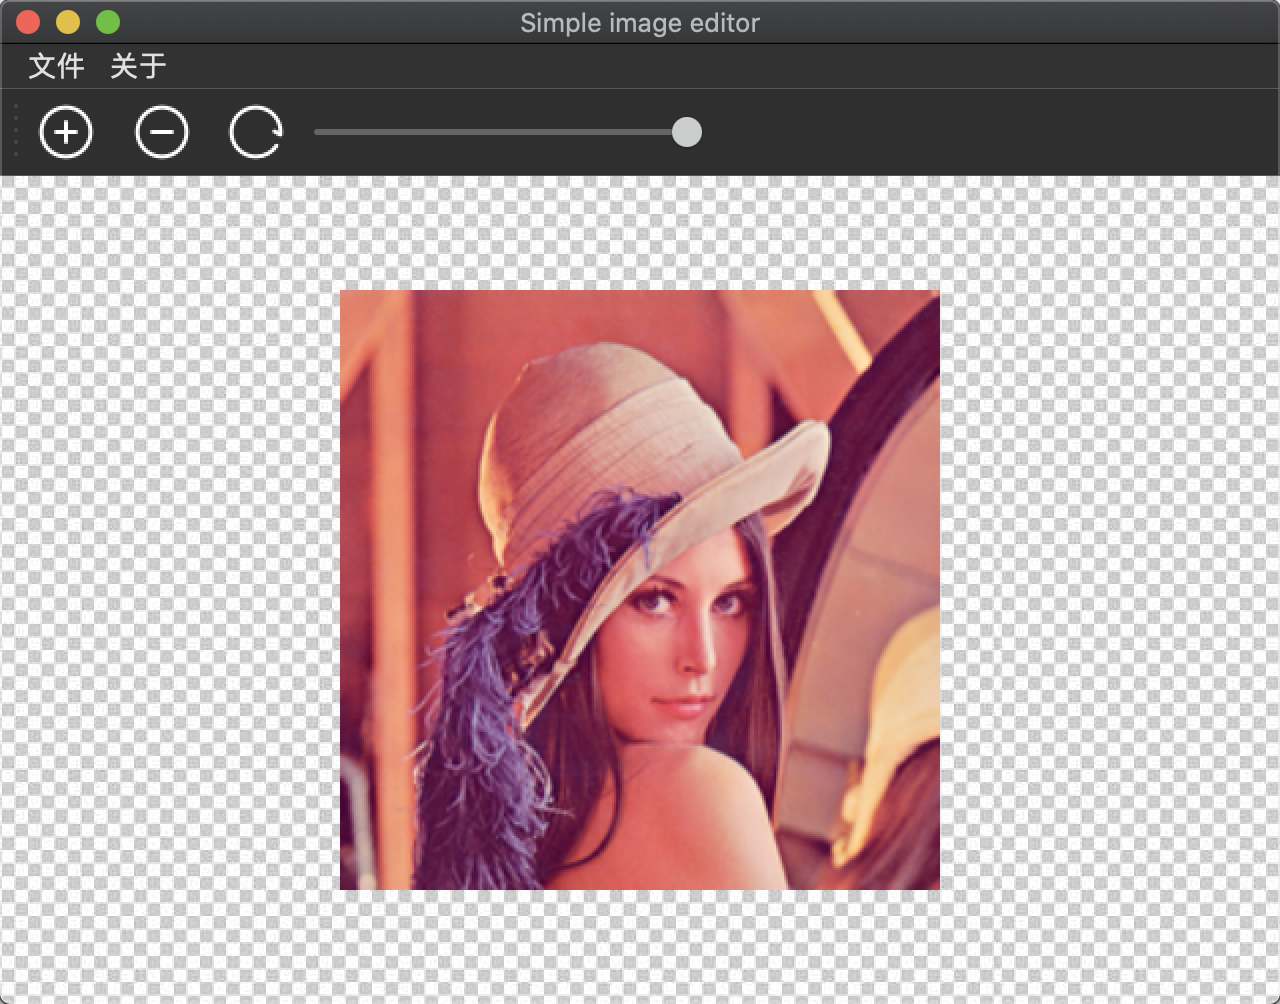
\includegraphics[keepaspectratio,alt={Image viewer}]{images/PyQt_image_viewer.png}}
\caption{Image viewer}
\end{figure}

一个比较典型的桌面程序，一个主界面包含菜单栏、工具栏、主界面，状态栏没有。这些都好理解，而另一个比较重要的概念是布局，就是控件在UI上怎么摆放（尤其是UI可能会缩放），通常不会是写死的位置，而是由布局管理器来管理。简而言之，就是定义规则，你的控件怎么放，窗口缩放的时候，怎么处理。

\subsection{主窗口}\label{ux4e3bux7a97ux53e3}

所以首先我们定义出主窗口。

\begin{Shaded}
\begin{Highlighting}[]
\KeywordTok{class}\NormalTok{ MainWindow(QMainWindow):}
    \KeywordTok{def} \FunctionTok{\_\_init\_\_}\NormalTok{(}\VariableTok{self}\NormalTok{, }\OperatorTok{*}\NormalTok{args, }\OperatorTok{**}\NormalTok{kwargs):}
        \BuiltInTok{super}\NormalTok{(MainWindow, }\VariableTok{self}\NormalTok{).}\FunctionTok{\_\_init\_\_}\NormalTok{(}\OperatorTok{*}\NormalTok{args, }\OperatorTok{**}\NormalTok{kwargs)}
        \VariableTok{self}\NormalTok{.setWindowTitle(}\StringTok{\textquotesingle{}Simple image editor\textquotesingle{}}\NormalTok{)}
        \VariableTok{self}\NormalTok{.setFixedSize(}\DecValTok{640}\NormalTok{, }\DecValTok{480}\NormalTok{) }\CommentTok{\# 固定大小的窗口，禁止缩放}
\end{Highlighting}
\end{Shaded}

实际上你可以直接显示一个其他控件例如QWidget, QLabel等，它们只是控件级别，而主窗口包含菜单、状态栏等，更适合制作程序UI。然后我们主界面的控件只有一个，那就是显示图片。图片可以使用QLabel显示，虽然它更多用来显示文字：

\begin{Shaded}
\begin{Highlighting}[]
\CommentTok{\# 在Qt里面，每一个控件都可以指定父控件，更多的是因为C++中需要自动管理内存}
\CommentTok{\# 当父控件销毁时，子控件跟着销毁，所以把self（主窗口）传给主窗口上的控件}
\VariableTok{self}\NormalTok{.imageContainer }\OperatorTok{=}\NormalTok{ QLabel(}\VariableTok{self}\NormalTok{)}
\VariableTok{self}\NormalTok{.imageContainer.setAlignment(Qt.AlignCenter)}

\CommentTok{\# qt可以写css来设置样式}
\VariableTok{self}\NormalTok{.imageContainer.setStyleSheet(}\StringTok{\textquotesingle{}background{-}image:url(background.jpg);\textquotesingle{}}\NormalTok{)}

\CommentTok{\# 将图片设置为中心控件}
\VariableTok{self}\NormalTok{.setCentralWidget(}\VariableTok{self}\NormalTok{.imageContainer)}
\end{Highlighting}
\end{Shaded}

\subsection{创建菜单和工具栏}\label{ux521bux5efaux83dcux5355ux548cux5de5ux5177ux680f}

菜单通过\texttt{self.menuBar}得到。

\begin{Shaded}
\begin{Highlighting}[]
\NormalTok{menu }\OperatorTok{=} \VariableTok{self}\NormalTok{.menuBar()}
\CommentTok{\# 是否使用系统菜单，如果是mac，不设置的话菜单会在屏幕顶上}
\NormalTok{menu.setNativeMenuBar(}\VariableTok{False}\NormalTok{)}
\NormalTok{aboutMenu }\OperatorTok{=}\NormalTok{ menu.addMenu(}\StringTok{\textquotesingle{}\&关于\textquotesingle{}}\NormalTok{)}
\NormalTok{aboutMenu.addAction(aboutAction) }
\end{Highlighting}
\end{Shaded}

工具栏跟菜单很类似，工具栏上的按钮都是一个Action，如果希望放进去别的控件可以用\texttt{addWidget}实现

\begin{Shaded}
\begin{Highlighting}[]
\CommentTok{\# 创建一个新的工具栏，可以创建多个}
\VariableTok{self}\NormalTok{.toolbar }\OperatorTok{=} \VariableTok{self}\NormalTok{.addToolBar(}\StringTok{\textquotesingle{}Operations\textquotesingle{}}\NormalTok{)}

\CommentTok{\# 图标按钮}
\NormalTok{zoomInAction }\OperatorTok{=}\NormalTok{ QAction(QIcon(}\StringTok{\textquotesingle{}zengjia.svg\textquotesingle{}}\NormalTok{), }\StringTok{\textquotesingle{}放大\textquotesingle{}}\NormalTok{, }\VariableTok{self}\NormalTok{)}
\VariableTok{self}\NormalTok{.toolbar.addAction(zoomInAction)}

\CommentTok{\# 非按钮控件}
\NormalTok{slider }\OperatorTok{=}\NormalTok{ QSlider(Qt.Horizontal)}
\NormalTok{slider.setFixedWidth(}\DecValTok{200}\NormalTok{)}
\VariableTok{self}\NormalTok{.toolbar.addWidget(slider)}
\end{Highlighting}
\end{Shaded}

\section{事件响应}\label{ux4e8bux4ef6ux54cdux5e94}

Qt是信号（Signal）/槽（Slot）机制，简单来说就是用户对界面的更改会产生事件，而事件由槽来处理，两者之间需要关联（connect）上才能正确处理。比如菜单的处理：

\begin{Shaded}
\begin{Highlighting}[]
\NormalTok{aboutAction }\OperatorTok{=}\NormalTok{ QAction(}\StringTok{\textquotesingle{}\&版本\textquotesingle{}}\NormalTok{, }\VariableTok{self}\NormalTok{)}
\NormalTok{aboutAction.setShortcut(}\StringTok{\textquotesingle{}Ctrl+A\textquotesingle{}}\NormalTok{)}
\CommentTok{\# triggered事件 关联到槽，槽就是一个函数}
\NormalTok{aboutAction.triggered.}\ExtensionTok{connect}\NormalTok{(}\VariableTok{self}\NormalTok{.onAbout)}
\end{Highlighting}
\end{Shaded}

有时候事件是会有参数的，比如滑块变化的时候，值是可以得到的：

\begin{Shaded}
\begin{Highlighting}[]
\NormalTok{slider }\OperatorTok{=}\NormalTok{ QSlider(Qt.Horizontal)}
\NormalTok{slider.setFixedWidth(}\DecValTok{200}\NormalTok{)}
\NormalTok{slider.setValue(}\DecValTok{100}\NormalTok{)}
\NormalTok{slider.valueChanged.}\ExtensionTok{connect}\NormalTok{(}\VariableTok{self}\NormalTok{.onChangeBrightness)}

\CommentTok{\# 槽}
\KeywordTok{def}\NormalTok{ onChangeBrightness(}\VariableTok{self}\NormalTok{, value):}
    \CommentTok{\# 这个value就是变化后的值（默认0{-}100）}
    \ControlFlowTok{pass}
\end{Highlighting}
\end{Shaded}

\section{图片处理}\label{ux56feux7247ux5904ux7406}

\subsection{放大缩小}\label{ux653eux5927ux7f29ux5c0f}

方法和缩小通过QPixmap.scaled来实现，我们通过将图片缩放到一个期望的大小（保持宽高比），来显示到界面上：

\begin{Shaded}
\begin{Highlighting}[]
\NormalTok{ scaledImage }\OperatorTok{=}\NormalTok{ rotatedImage.scaled(}\VariableTok{self}\NormalTok{.imageSize.width(), }\VariableTok{self}\NormalTok{.imageSize.height(), Qt.KeepAspectRatio, Qt.SmoothTransformation)}
\VariableTok{self}\NormalTok{.imageContainer.setPixmap(scaledImage)}
\end{Highlighting}
\end{Shaded}

而缩放的时候，实际上就是在控制这个大小：

\begin{Shaded}
\begin{Highlighting}[]
\CommentTok{\# 一开始给定一个默认的大小}
\VariableTok{self}\NormalTok{.imageSize }\OperatorTok{=}\NormalTok{ QSize(}\DecValTok{300}\NormalTok{, }\DecValTok{200}\NormalTok{)}

\KeywordTok{def}\NormalTok{ onZoomOut(}\VariableTok{self}\NormalTok{):}
    \CommentTok{\# 缩小按0.5计算，扩大按照乘以1.5计算}
    \VariableTok{self}\NormalTok{.imageSize }\OperatorTok{*=} \FloatTok{0.5}
    \VariableTok{self}\NormalTok{.refreshImage()}
\end{Highlighting}
\end{Shaded}

\subsection{旋转}\label{ux65cbux8f6c}

旋转需要记录一个旋转角度，然后通过Qtransform来实现：

\begin{Shaded}
\begin{Highlighting}[]
\NormalTok{transform }\OperatorTok{=}\NormalTok{ QTransform()}
\NormalTok{transform.rotate(}\VariableTok{self}\NormalTok{.rotateAngle)}
\NormalTok{rotatedImage }\OperatorTok{=} \VariableTok{self}\NormalTok{.image.transformed(transform)}
\end{Highlighting}
\end{Shaded}

这样可以得到一个新的QPixmap，就是旋转后的图片。

\subsection{调节亮度}\label{ux8c03ux8282ux4eaeux5ea6}

亮度调节就比较麻烦了，图片的亮度调节需要在HSL的颜色空间下处理（我们比较熟悉的一帮是RGB三色表示）。

\begin{Shaded}
\begin{Highlighting}[]
\CommentTok{\# 将QPixmap转为QImage，以便可以直接操作像素}
\NormalTok{image }\OperatorTok{=} \VariableTok{self}\NormalTok{.rawImage.toImage()}
\ControlFlowTok{for}\NormalTok{ i }\KeywordTok{in} \BuiltInTok{range}\NormalTok{(}\DecValTok{0}\NormalTok{, image.width()):}
    \ControlFlowTok{for}\NormalTok{ j }\KeywordTok{in} \BuiltInTok{range}\NormalTok{(}\DecValTok{0}\NormalTok{, image.height()):}
        \CommentTok{\# 取到(i, j)位置的像素点}
\NormalTok{        color }\OperatorTok{=}\NormalTok{ QColor(image.pixelColor(i, j))}

        \CommentTok{\# 取到HSL空间下的像素值}
\NormalTok{        (h, s, l, a) }\OperatorTok{=}\NormalTok{ color.getHsl()}

        \CommentTok{\# 计算调整后的亮度值并更新，更新的时候转成了rgb}
\NormalTok{        newBrightless }\OperatorTok{=}\NormalTok{ l }\OperatorTok{*}\NormalTok{ (value}\OperatorTok{/}\FloatTok{100.0}\NormalTok{)}
\NormalTok{        color.setHsl(h, s, newBrightless, a)}
\NormalTok{        image.setPixel(i, j, color.rgb())}
\VariableTok{self}\NormalTok{.image }\OperatorTok{=}\NormalTok{ QPixmap.fromImage(image)}
\end{Highlighting}
\end{Shaded}

以上就是一个简单的例子，完整的程序\href{/images/ImageEditor.zip}{下载}：


\end{document}
